\begin{frame}{Les notions abordées}
    \begin{itemize}
        \item Auto-édition
        \item Auto-publication
        \item Publications à compte d'auteur
    \end{itemize}
\end{frame}

\begin{frame}{Publication à compte d'auteur}
    Consiste pour un auteur à faire éditer ses propres ouvrages \textbf{par un éditeur qui assure seulement la partie technique de l'édition et de la diffusion.}\\
    \textrightarrow{} L'auteur paie les frais d'impression et de publicité mais reste propriétaire de ses droits d'auteur.\\
\end{frame}

\begin{frame}{Publication à compte d'auteur}
    \begin{columns}
    % Colonne de gauche : Texte
        \begin{column}{0.4\textwidth}
            \begin{itemize}
                \item Système inventé par \textbf{Bernard Grasset}.
                \item Créateur du marketing éditorial.
                \item Exemple de Proust en 1913: 1250 exemplaires du premier tome sont imprimés.
            \end{itemize}
        \end{column}

        % Colonne de droite : Image
        \begin{column}{0.5\textwidth}
            \centering
            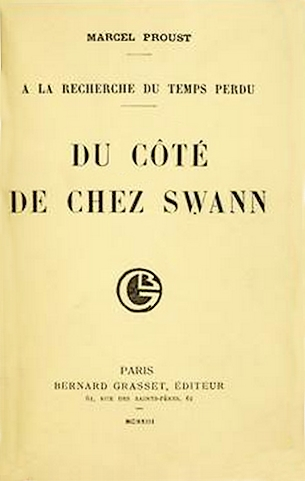
\includegraphics[width=.70\columnwidth]{images/Proust_1913.jpg}
        \end{column}
    \end{columns}
\end{frame}

\begin{frame}{Publication à compte d'auteur}
    \begin{itemize}
        \item \textbf{Le texte ne passe pas devant un comité de lecture} mais intègre tout de suite le circuit de fabrication;
        \item \textbf{L'éditeur n'assume pas le risque éditorial} \textrightarrow{} En contrepartie, l’auteur ne lui cède pas ses droits;
        \item \textbf{L'écrivain ne bénéficie pas tout à fait de la fonction de légitimation}: pas d'approbation d'un comité éditorial mais bénéficie des compétences techniques de fabrication du livre et de l'énonciation éditoriale.
    \end{itemize}

\end{frame}

\begin{frame}{Publication à compte d'auteur}
    \begin{columns}
    % Colonne de gauche : Texte
        \begin{column}{0.4\textwidth}
            \begin{itemize}
                \item Harmattan: fondée en 1975;
                \item Publication d'ouvrage d'auteurs africains ou tiers-mondistes;
                \item Permet d'éditer son livre gratuitement mais ne verse des droits d'auteurs qu'à partir du 500ème livre vendu.
            \end{itemize}
        \end{column}

        % Colonne de droite : Image
        \begin{column}{0.5\textwidth}
            \centering
            
\includegraphics[width=\textwidth]{images/harmattan.png}
        \end{column}
    \end{columns}
\end{frame}

\begin{frame}{Auto-publication}
    Consiste à rendre public un texte, sans nécessairement cherche à le commercialiser.\\
    \textrightarrow{} Impact du développement du web à compter des années 1990.
\end{frame}
\begin{frame}{Auto-publication et édition numérique : naissance d'une nouvelle avant-garde littéraire}
    Rappel:
    \begin{itemize}
        \item Web = application d'internet, qui propose une infrastructure en réseau et permet de publier des contenus de tous types.
        \item Textes publiés sur le Web dès les années 90 sont des textes encodés dans des formats numériques: XML, HTML.
    \end{itemize}
    \textbf{Naissance d'un web littéraire \textrightarrow{} avant-garde littéraire:}
    \begin{itemize}
        \item Écrivains des débuts du web doivent apprendre des langages de programmation.
        \item Vont créer des oeuvres littéraires qui reposent non seulement sur le langage naturel, mais aussi sur une exploitation du langage de progammation.
    \end{itemize}
    
\end{frame}

\begin{frame}{Des outils pour l'auto-publication}
    \begin{columns}
    % Colonne de gauche : Texte
        \begin{column}{0.4\textwidth}
            \begin{itemize}
                \item Années 2000: multiplication d'outils de publication;
                \item Directement possible de publier un contenu sur le web sans connaître HTML, CSS ou Javascript.
            \end{itemize}
        \end{column}

        % Colonne de droite : Image
        \begin{column}{0.5\textwidth}
            \centering
            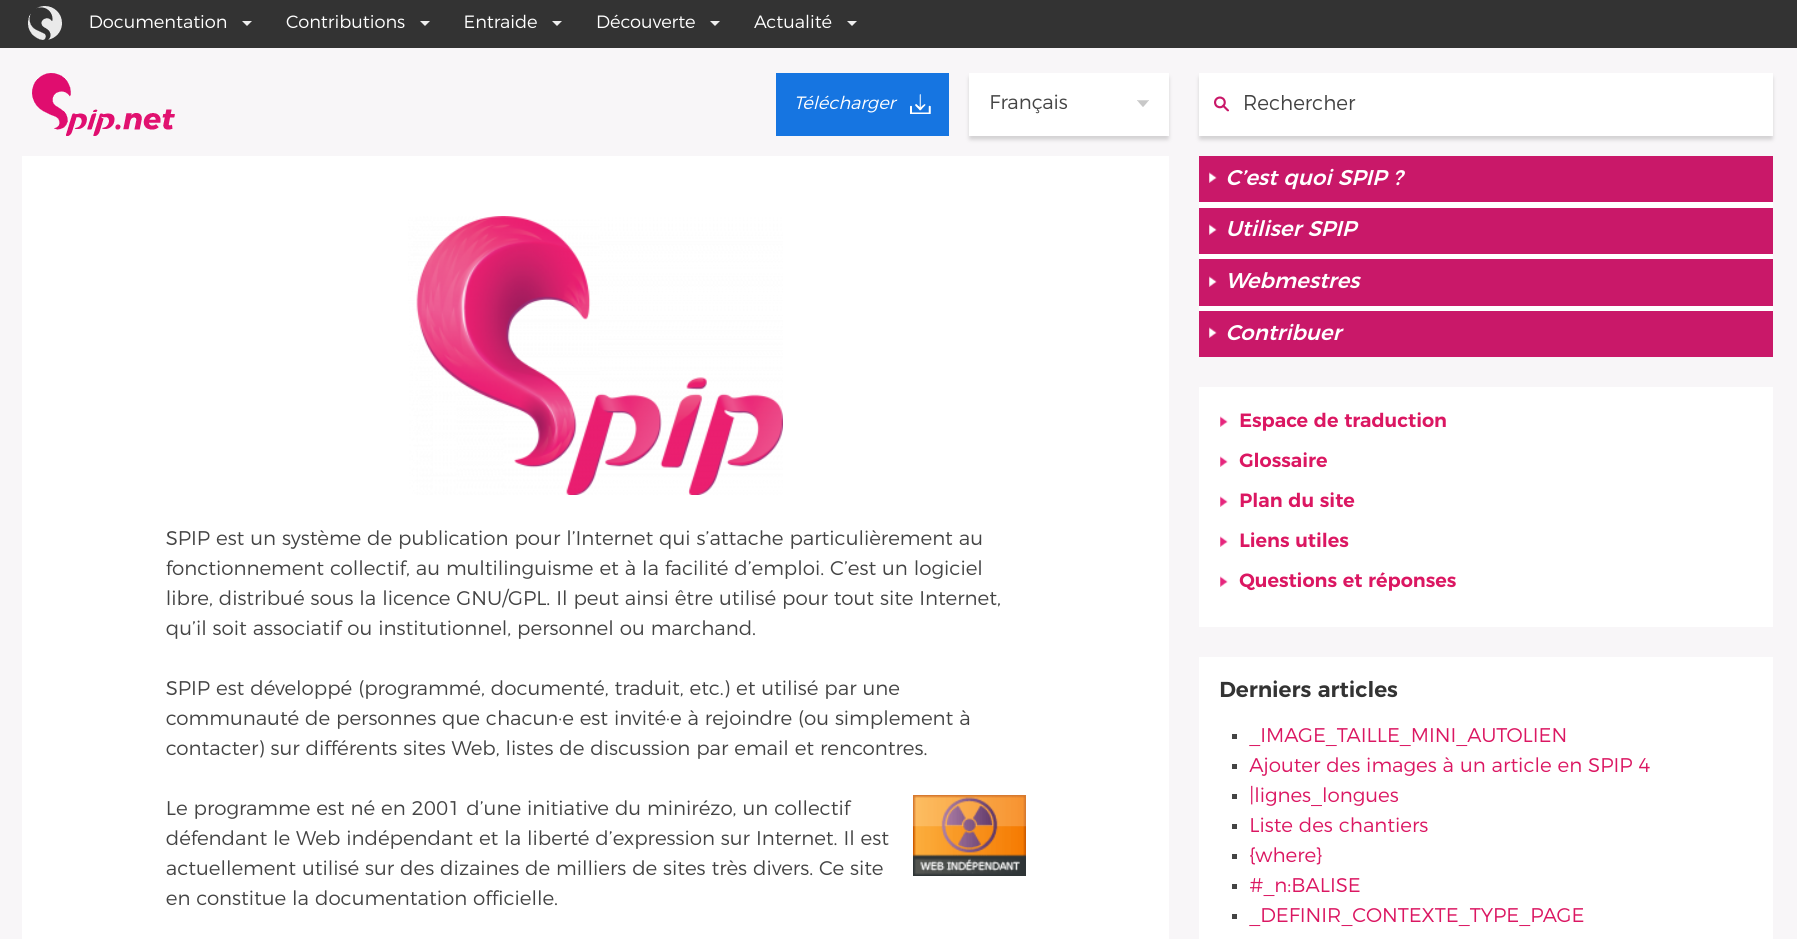
\includegraphics[width=\textwidth]{images/spip1.png}
        \end{column}
    \end{columns}
\vspace{2em}
\textbf{Sur la souveraineté des outils:} question des modèles économiques de l'édition numérique (les GAFAM) \textrightarrow{} Nouveau monopole éditorial qui ne rémunère pas ce qui est publié par exemple. 
\end{frame}
\begin{frame}{Les "plateformes littéraires"}
    \begin{columns}
    % Colonne de gauche : Texte
        \begin{column}{0.4\textwidth}
            \begin{itemize}
                \item Plateformes dédiées de type Wattpad;
                \item Des outils de plus en plus formattés;
                \item Des degrès de "professionnalisme" variables. Wattpad revendique l'amateurisme par exemple.
            \end{itemize}
        \end{column}

        % Colonne de droite : Image
        \begin{column}{0.5\textwidth}
            \centering
            
\includegraphics[width=\textwidth]{images/wattpad.png}
        \end{column}
    \end{columns}
\end{frame}

\begin{frame}{Les "plateformes littéraires"}
    \begin{columns}
    % Colonne de gauche : Texte
        \begin{column}{0.4\textwidth}
            \begin{itemize}
                \item écosystèmes de publication: kindle direct publishing, kobo writing life, iBooks authors\dots
                \item Ne demandent aucune contribution financière à l’auteur mais le travail éditorial n'est pas pris en charge.
            \end{itemize}
        \end{column}

        % Colonne de droite : Image
        \begin{column}{0.5\textwidth}
            \centering
            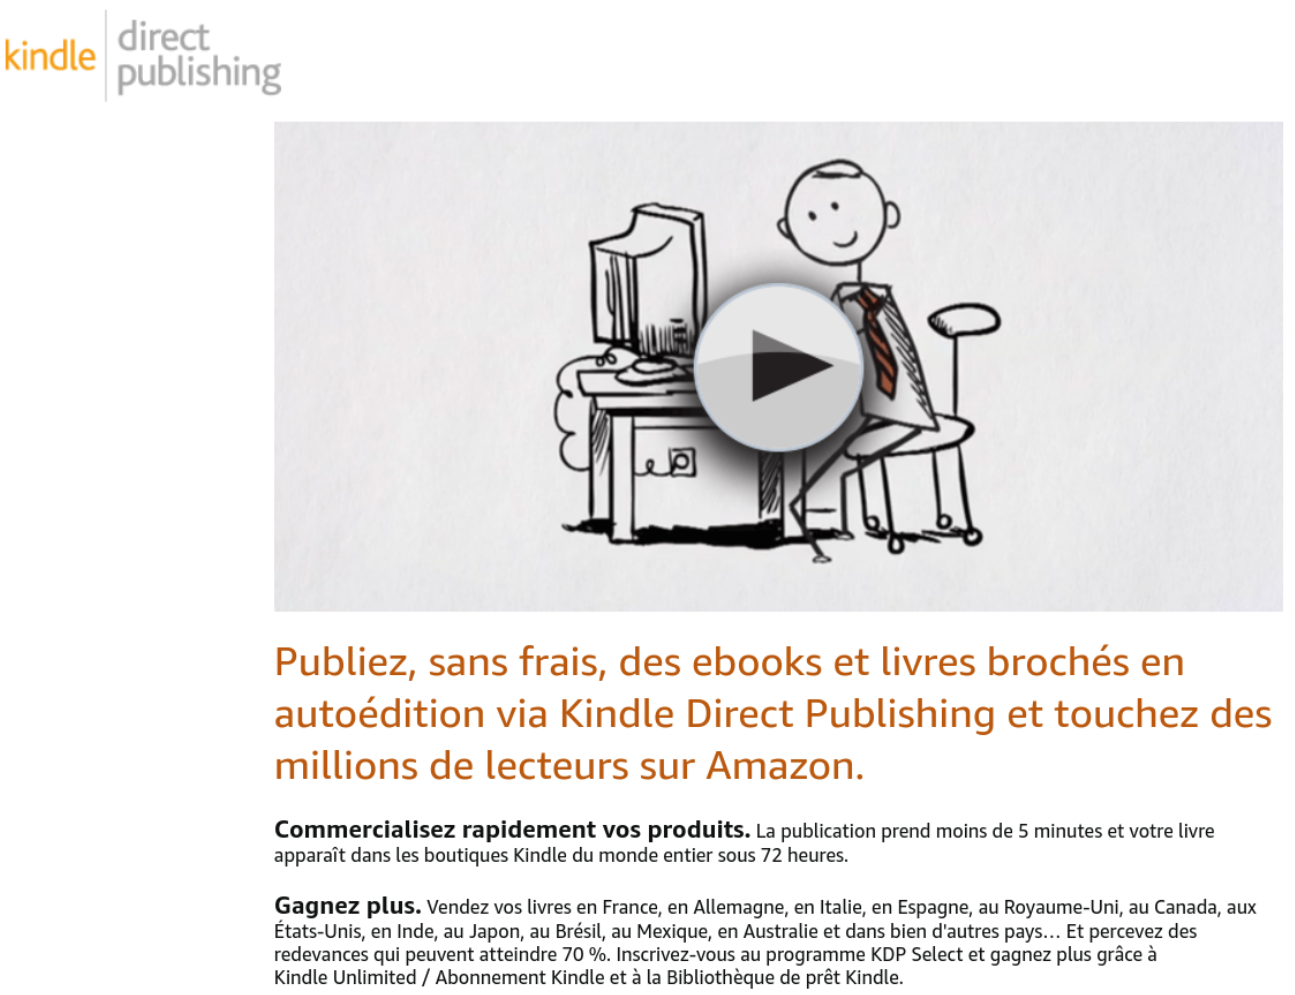
\includegraphics[width=\textwidth]{images/kindle_publishing.png}
        \end{column}
    \end{columns}
    
\end{frame}

\begin{frame}{Quelques \textit{success stories} qui alimentent les fantasmes}
    \begin{figure}
        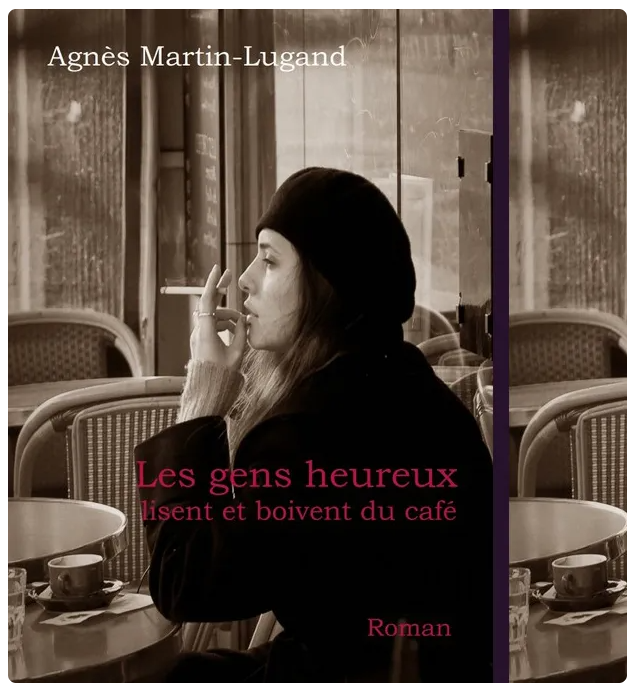
\includegraphics[width=.60\textwidth]{images/AgnesMartinLugand.png}
    \end{figure}
    
\end{frame}
\begin{frame}{Quelques \textit{success stories} qui alimentent les fantasmes}
    \begin{columns}
    % Colonne de gauche : Texte
        \begin{column}{0.4\textwidth}
            \begin{itemize}
                \item Exemple d'éditeurs-diffuseurs numériques: Librinova.
                \item Propose contre rémunération un accompagnement de l'auteur sous la forme de prestations professionnelles.
            \end{itemize}
        \end{column}

        % Colonne de droite : Image
        \begin{column}{0.5\textwidth}
            \centering
            
\includegraphics[width=\textwidth]{images/librinova.png}
        \end{column}
    \end{columns}
    
\end{frame}
\begin{frame}{Auto-édition}
    Renvoie à un modèle d'auto-publication: 
    \begin{itemize}
        \item qualitatif
        \item Modèle éditorial traditionnel
        \item Souvent une vocation marchande.
    \end{itemize}
    
\end{frame}
\begin{frame}{Exemple: Tiers Livre éditeur de François Bon}
    \begin{figure}
        \centering
        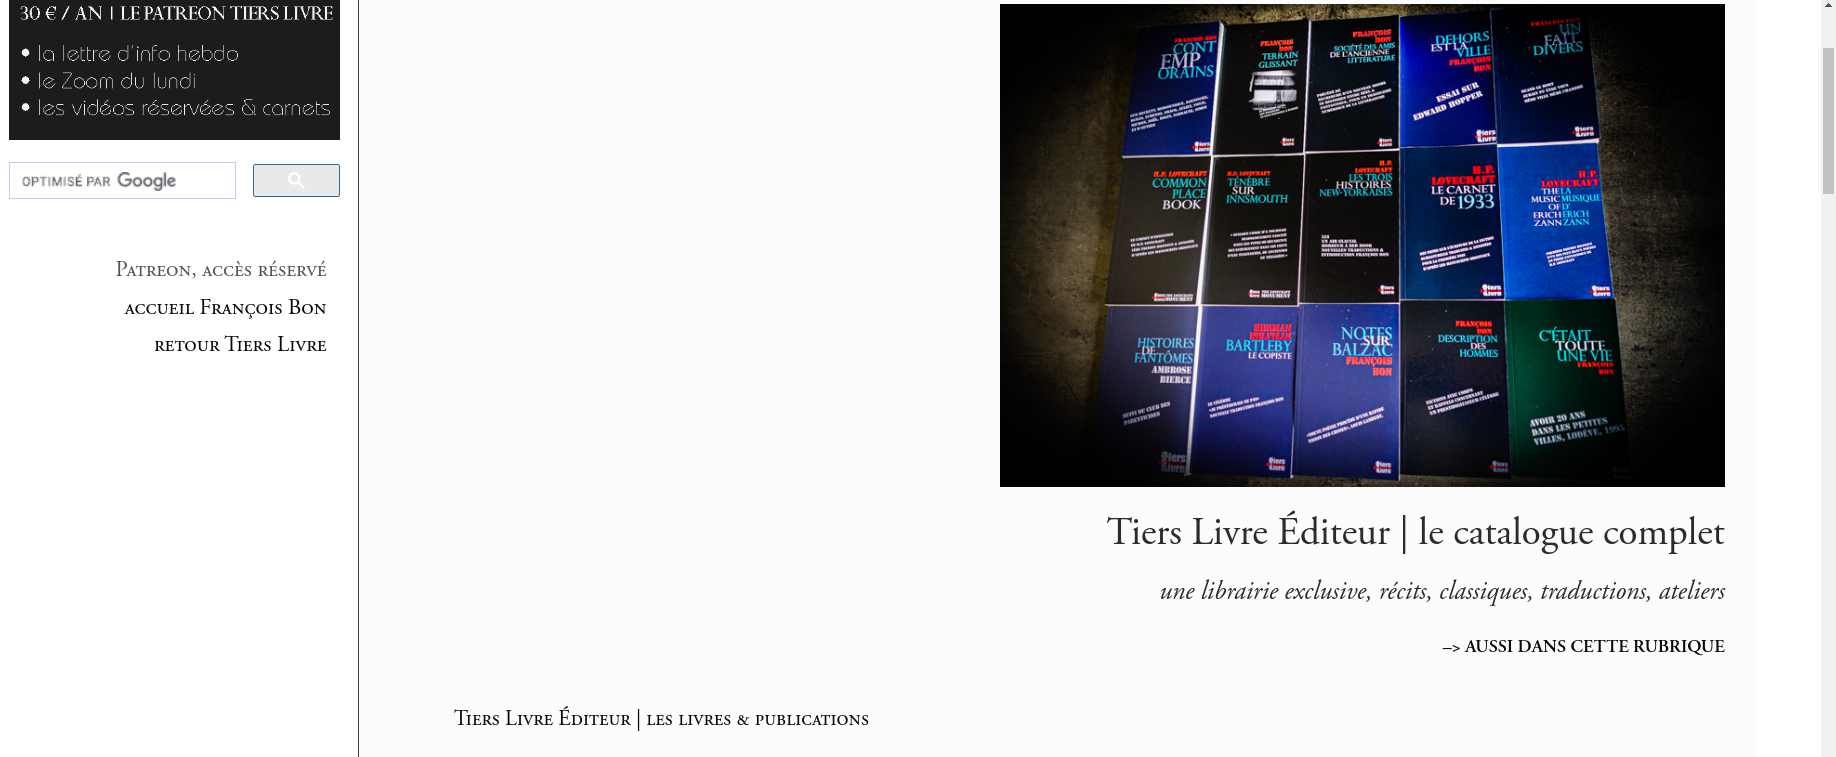
\includegraphics[width=.4\textwidth, height=3cm]{images/FBediteur.png}
        \hspace{1em}
        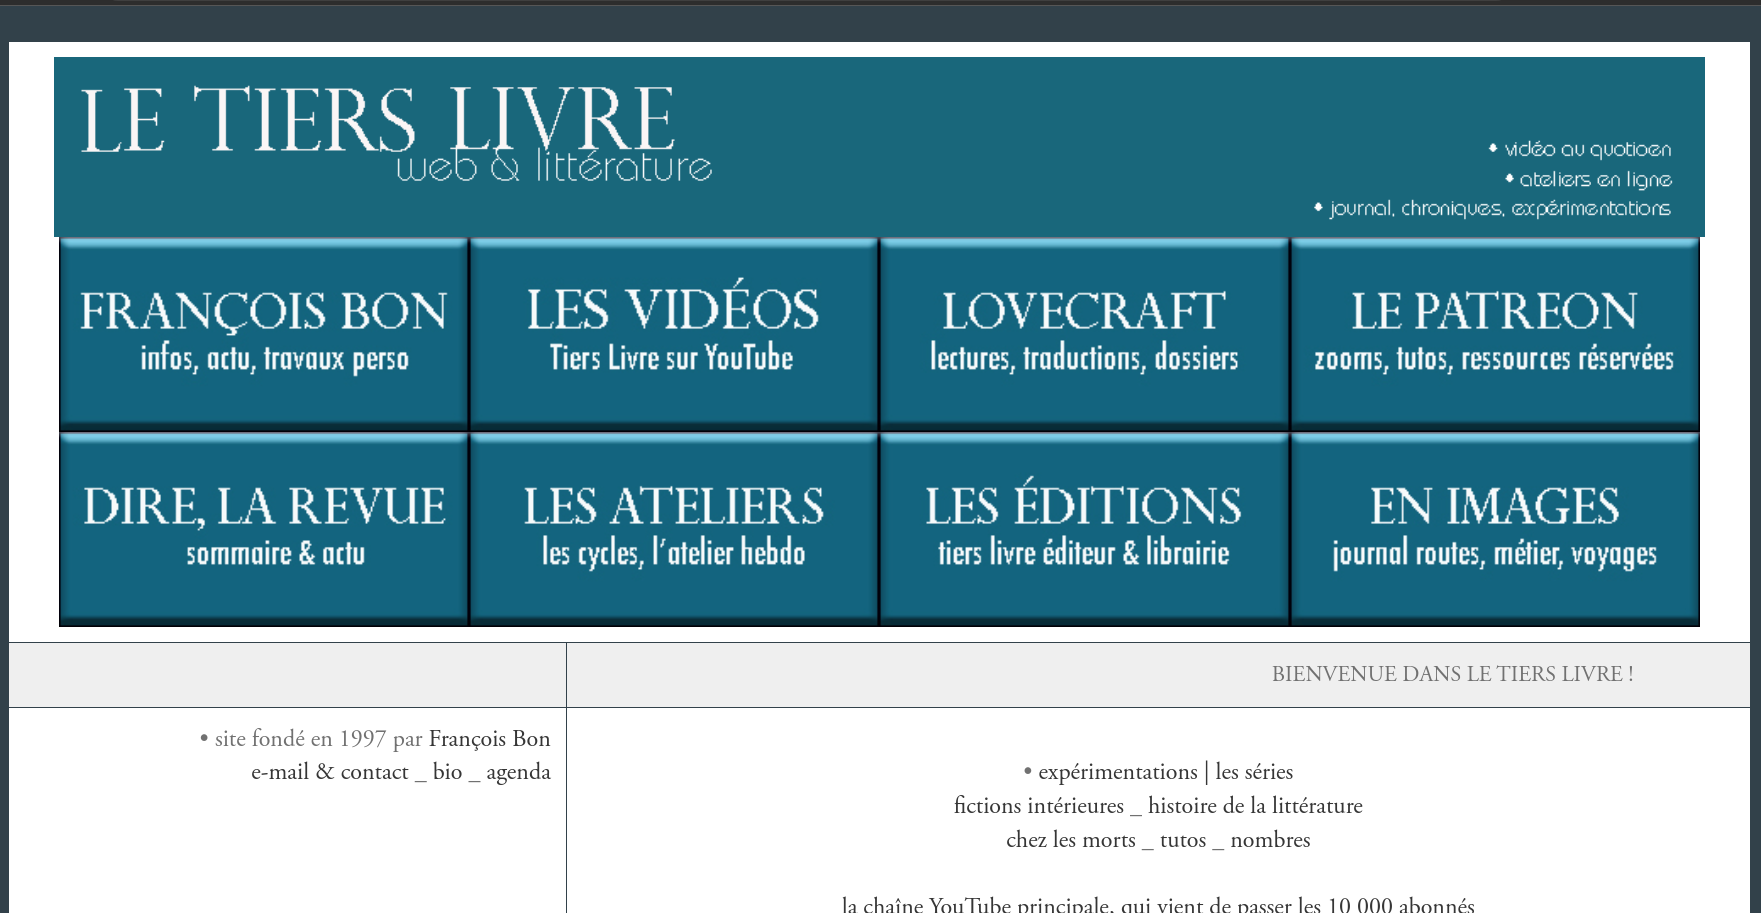
\includegraphics[width=.4\textwidth]{images/FBediteur2.png}
    \end{figure}
\end{frame}

\begin{frame}{Autre exemple: Pierre Ménard de La Marelle au livre-objet auto-édité}
    \begin{figure}
        \centering
        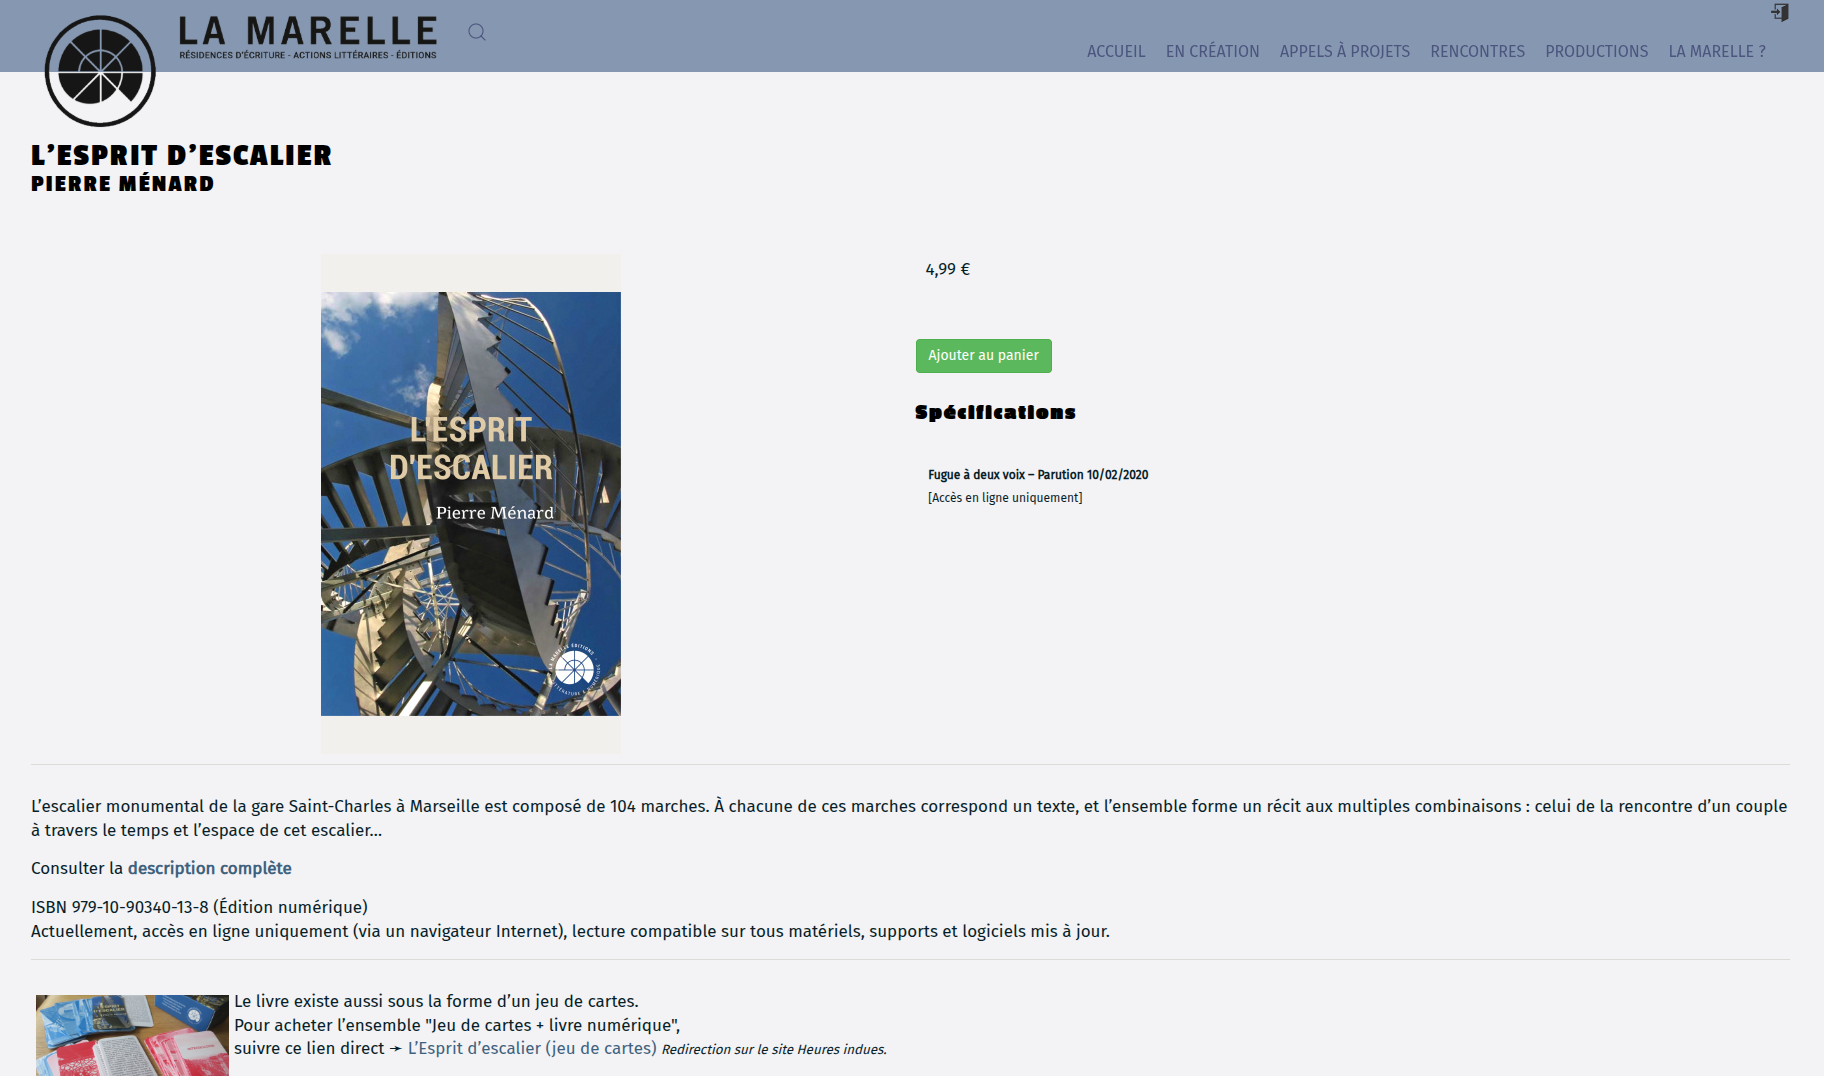
\includegraphics[width=.4\textwidth]{images/espritEscalier.png}
        \hspace{1em}
        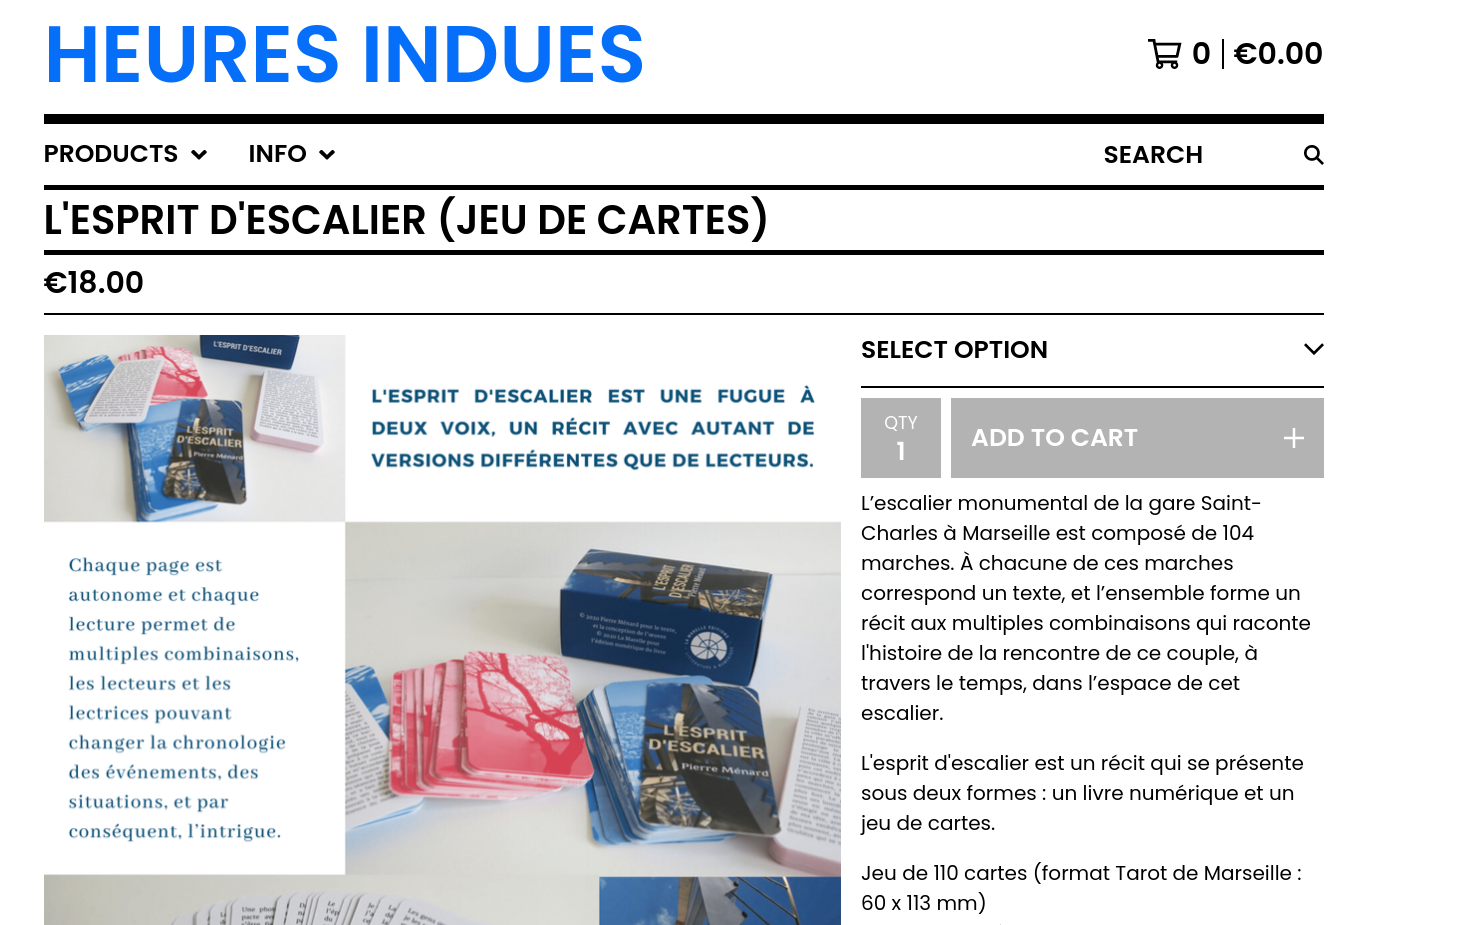
\includegraphics[width=.4\textwidth]{images/heuresIndues.png}
    \end{figure}
\end{frame}